\documentclass[a4paper,10pt]{article}

\usepackage[utf8]{inputenc}
\usepackage{natbib}
\usepackage[margin=0.48in]{geometry}
\geometry{tmargin=0.0in}
\setlength{\bibsep}{1pt}
\renewcommand{\bibfont}{\small}

\usepackage{caption}
\usepackage{subcaption}
\usepackage{graphicx}
\usepackage{float}

\graphicspath{ {Figures/} }

\title{Project proposal - Probabilistic graphical models}
\author{Xi SHEN, Othman SBAI, Chaimaa KADAOUI}
\date{Dec, 2016}


\begin{document}
\maketitle
\section{Motivation: subject introduction}
A Restricted Boltzmann Machine (RBM) is a undirected energy-based probabilistic graphical model which can be seen as a two layer neural network (visible and hidden units). RBMs can be used to model and learn important aspects of a probability distribution of a training data. They are called restricted, because we impose restrictions on the network topology, by allowing only connections between units of different layers. RBM are energy-based, since they define probability distribution through an energy function. Learning corresponds to shaping the energy so that desirable configurations have a low energy and thus maximize probability of training data under the model. Maximum likelihood learning is challenging for undirected graphical models because MLE parameters cannot be found analytically and the log likelihood gradient based optimization is not tractable. This optimization requires obtaining samples through Markov Chain Monte Carlo, which is computationally demanding.\cite{hinton2010practical},\cite{tieleman2008training},\cite{fischer2014training}

\section{Operational organization}
\subsection{Plan of work}
\begin{itemize}
    \setlength{\itemsep}{3pt}
    \setlength{\parskip}{0pt}
    \item Theory of Restricted Boltzmann Machines, and advanced training techniques
	\item Implementing RBM on MNIST data in python
	\item Compare the performance speedup using a deeplearning library (TensorFlow)
	\item Experimenting how RBM training depends on different parameters (learning rate, batch size, Contrastive divergence steps, number of hidden units...)
	\item Experimenting on robustness of RBM learning (white or black background, image translation..)
\end{itemize}

\subsection{Expected work sharing}

\begin{itemize}
    \setlength{\itemsep}{3pt}
    \setlength{\parskip}{0pt}
    %Python implementation
    \item Xi will be focused on the work regarding the python implementation of RBM running on CPU, experimenting on different values such as learning rate, n hidden layers, batch size, n CD steps...
    %Tensorflow implementation
	\item Othman will focus on the comparing the performance of the python implementation with tensorflow one. 
	%Robustness of developed algorithms
	\item Finally, Chaïmaa will work on assessing the robustness of RBM algorithm with respect to background change (black and white)
	\item Other applications of RBM will be tackled depending on advancement. 
\end{itemize}

\section{First results}

Training the RBM model on MNIST data, with parameters (learning rate = 0.001, batch size = 100, n hidden units = 100). After 100 epoch of training we obtain the following samples fig:~\ref{samples}. At the first iterations, we had random black and white pixels for the generated samples. After 100 iterations, we can see that the model starts learning the distribution of the data, since it has become able to generate images looking like hand-written digits.

\begin{figure}[H]
    \centering
    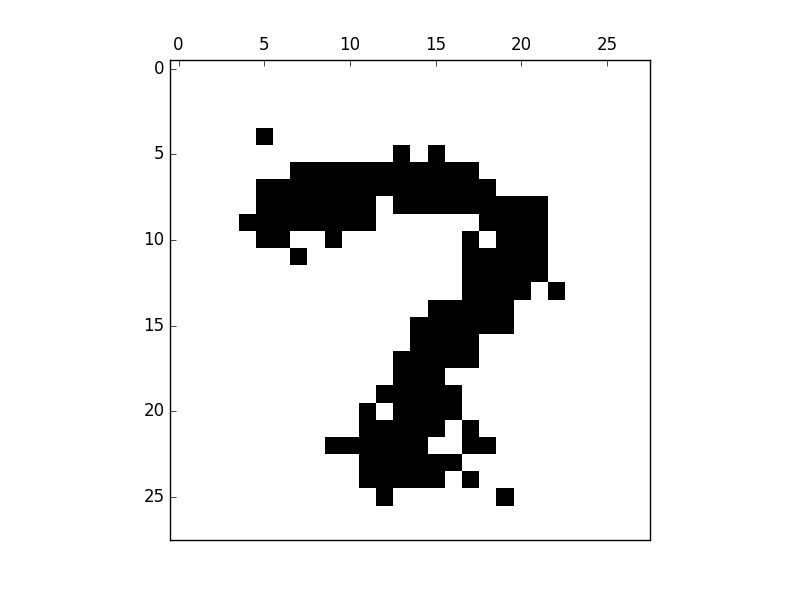
\includegraphics[width=0.15\linewidth]{sample0_at_epoch100}
    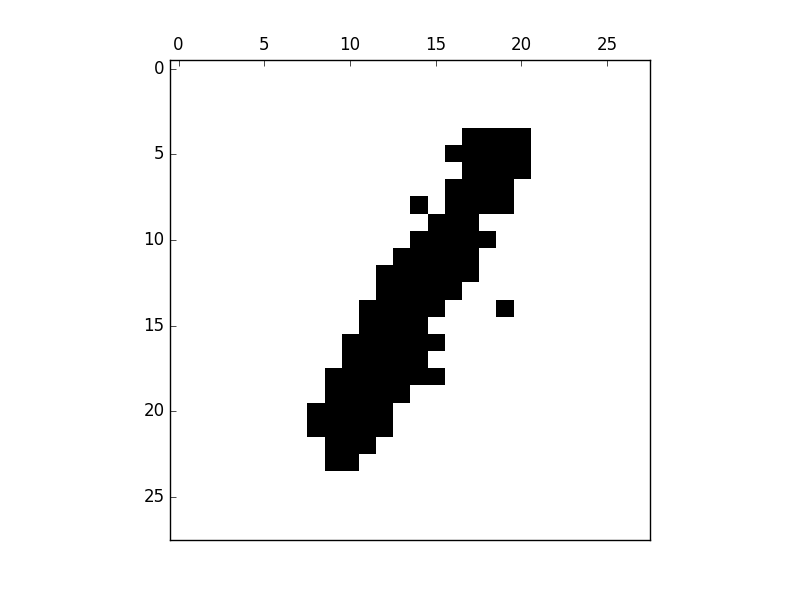
\includegraphics[width=0.15\linewidth]{sample2764_at_epoch100}
    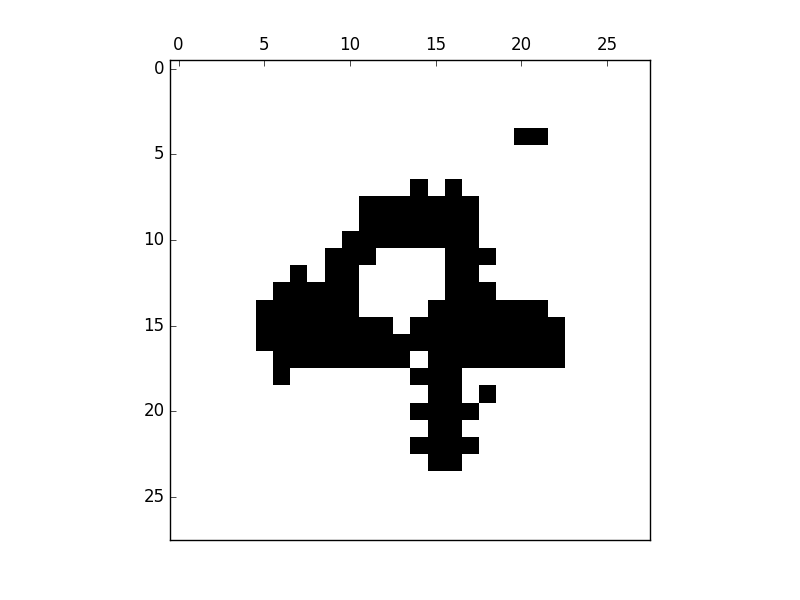
\includegraphics[width=0.15\linewidth]{sample31227_at_epoch100}
    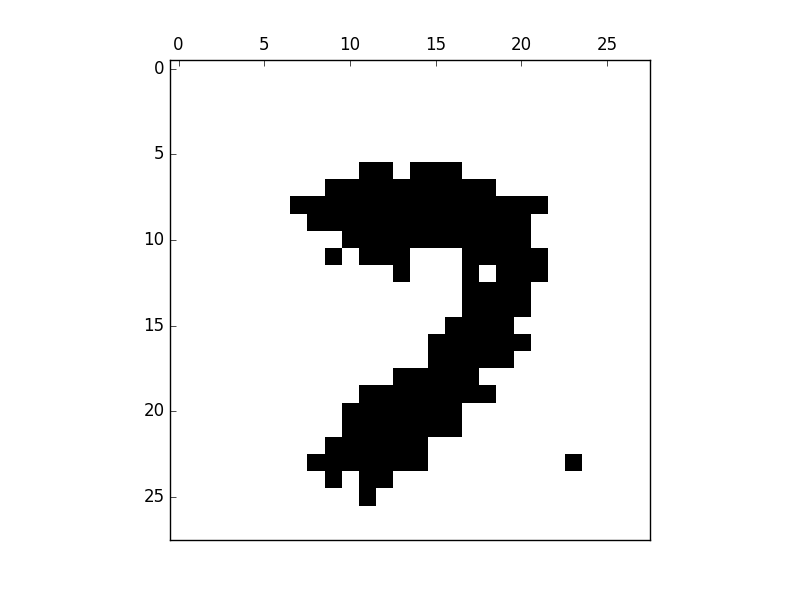
\includegraphics[width=0.15\linewidth]{sample44983_at_epoch100}
    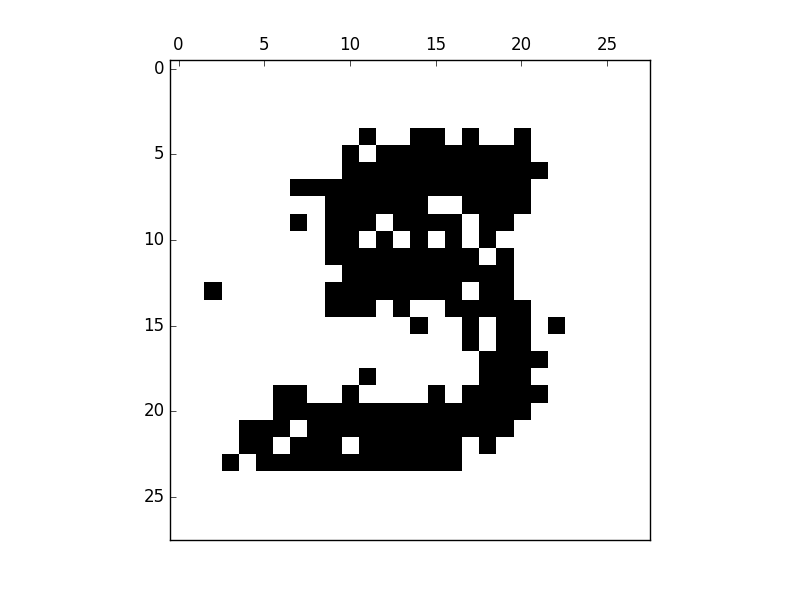
\includegraphics[width=0.15\linewidth]{sample72_at_epoch100}
    \caption{Generated samples After 100 epochs}
    \label{samples}
\end{figure}

\bibliography{biblio}
\bibliographystyle{plain}


\end{document}

\begin{thebibliography}{9}
	\setlength{\parskip}{0pt} 
	
	\bibitem{praticalGuide} Hinton G. \textit{ A practical guide to training restricted Boltzmann machines[J]. Momentum, 2010, 9(1): 926.}
	
	\bibitem{these} Fischer A. \textit{Training restricted boltzmann machines[J]. KI-KÃŒnstliche Intelligenz, 2015, 29(4): 441-444.}

	\bibitem{reviewArticle}  Bengio, Y., Delalleau, O. \textit{Justifying and generalizing contrastive divergence}. Neural Computation 21(6), 1601n621 (2009)
	
\end{thebibliography}
